%!TEX root = ClementiCooperBarba2018.tex

\subsection{Isolated nanoparticle} \label{sec:verification}

In the long-wavelength limit, the electrostatic approximation applies and
the electromagnetic scattering of a small spherical particle can be modeled
by a sphere in a constant electric field. 
Figure \ref{fig:np_elec_field} illustrates this scenario.

%
\begin{figure}[h] %  figure placement: here, top, bottom, or page
   \centering
   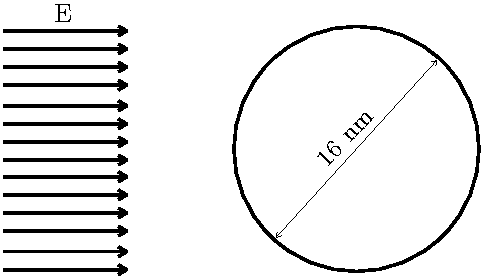
\includegraphics[width=0.3\textwidth]{sphere_field_8nm.pdf} 
   \caption{Spherical nanoparticle in a constant electric field.}
   \label{fig:np_elec_field}
\end{figure}
%

This model problem has an analytical solution, which allows us to compare with
the numerical calculations of the extinction cross-section obtained with \pygbe,
for code verification and grid-convergence analysis.
Mishchenko \cite{Mishchenko2007} derived the following analytical result, 
valid for lossy mediums:
%
\begin{equation} 
    C_\text{ext} = \frac{4\pi a^3}{k^\prime} \operatorname{Im}\left(k^2 
                    \frac{\epsilon_p/\epsilon_m -1}{\epsilon_p/\epsilon_m +2}\right),
    \label{eq:an_sol}
\end{equation}
%
Here, $a$ is the radius of the sphere, $k$ is the complex wave number ($k=k^\prime +i k^{\prime\prime}$), $\epsilon_p$ 
is the dielectric constant of the particle, and $\epsilon_m$ is the dielectric constant
of the host medium. If the medium is not lossy, then $k^{\prime\prime}=0$ and $k=k^\prime$.

We completed a grid-convergence study of \pygbe for the extinction
cross-section of a spherical silver nanoparticle of radius $8 \, nm$, immersed in water
under a z-polarized electric field with a wavelength of $380 nm$ and intensity of 
$-0.0037 e/({\AA}^2 \, \epsilon_0)$. In such conditions, water has a dielectric
constant of $1.7972 \, + \, 8.5048^{-09}i$ \cite{JohnsonChristy1972} and silver of
$-3.3877 \, + \, 0.1922i$ \cite{HaleQuerry1972}. These simulations use $K=4$ 
Gauss quadrature points per far-away elements, $K_{fine} = 37$ Gauss quadrature points
per elements for near singular integrals, $Nk = 9$ Gauss quadrature points per 
triangle edge for semi-analytical integration in the singular elements, $P=15$ for 
the order of expansion in treecode, and a GMRES tolerance of $10^{-5}$. We
performed the calculations using meshes with 512, 2048, 8192 and 32768 elements. For this case, the 
analytical solution in equation \eqref{eq:an_sol} yields $C_{ext} = 1854.4765 \; nm^2$.
Errors are also presented in Table \ref{table:err_iso_sphere}.

\begin{figure}[h] %  figure placement: here, top, bottom, or page
   \centering
   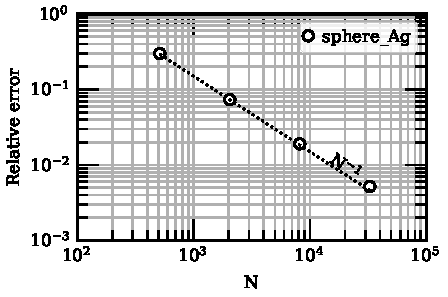
\includegraphics[width=0.45\textwidth]{convergence_sph_Ag_R8_w=380.pdf} 
   \caption{Grid-convergence study of extinction cross-section of a spherical silver
            nanoparticle.}
   \label{fig:error_sphere_Ag}
\end{figure}

The observed order of convergence is $0.98$, and the $1/N$ slope in Figure \ref{fig:error_sphere_Ag}
is an indication that the meshes are correctly resolving the numerical solutions with \pygbe. 

\begin{table}[h]
    \centering
    \caption{\label{table:err_iso_sphere} Percentage error of isolated silver sphere.} 
    \begin{tabular}{c c}
    \hline%\toprule
    N & \% error \\
    \hline%\midrule
     $512$ & $29.86$ \\
     $2048$ & $7.33$ \\
     $8192$ & $1.9$ \\
     $32768$ & $0.52$ \\
    \hline%\bottomrule
    \end{tabular}
\end{table}

We further verified our implementation computing the extinction cross-section of the 
isolated sphere for a range of wavelengths, presented in Figure \ref{fig:verif_sphere}. 
The mesh in these simulations had $N=32768$, which yields errors below $2\%$ in Table \ref{table:err_iso_sphere}.
The values of dielectric constants for each wavelength were obtained by interpolation of 
experimental data \cite{JohnsonChristy1972, HaleQuerry1972}.

\begin{figure}[h] %  figure placement: here, top, bottom, or page
   \centering
   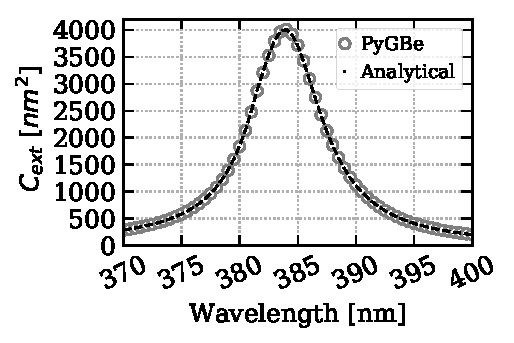
\includegraphics[width=0.45\textwidth]{silver_NP_verification.pdf} 
   \caption{Extinction cross-section as a function of wavelength for a $8 \, nm$
            silver sphere immersed in water.}
   \label{fig:verif_sphere}
\end{figure}

Figure \ref{fig:verif_sphere} shows good agreement between simulations and analytical results, proving
that \pygbe is accurately representing the mathematical model. The 
peak in the extinction cross-section indicates that the plasmons of the metallic
nanoparticle are resonating with the incoming electric field.


\subsection{LSPR response to BSA} \label{sec:lspr_response}

Localized Surface Plasmon Resonance (LSPR) biosensors detect a target molecule by monitoring
plasmon resonance frequency shifts of metallic nanoparticles, in presence of an analyte \cite{WilletsVandyune2007}.
In this section, we use our BEM approach to model the response of LSPR biosensors.
We consider a spherical silver nanoparticle, and compute the extinction cross-section placing 
bovine serum albumina (BSA) proteins (PDB code: 4FS5) in different locations.
The BSA mesh was generated using the open source software Nanoshaper \cite{Nanoshaper}. 
Nanoshaper takes as inputs the atomic coordinates and radii, which were 
extracted from a \texttt{pqr} file generated with \texttt{pdb2pqr} \cite{Dolinsky04},
 using the built-in \texttt{amber} force field.

\subsubsection{Grid-convergence study} \label{sec:bsa_convergence}
To guarantee an accurate numerical solution, we performed a grid-convergence 
analysis of the system sketched in Figure \ref{fig:setup_conv}. 
Since we compute the extinction cross-section of the spherical nanoparticle only, we 
set a fixed mesh density for the protein and refined the mesh of the
sphere (meshes of 512, 2048, 8192 and 32768 elements). We found that the protein meshed with two
triangles per ${\AA}^2$ was fine enough for the convergence analysis, resulting in $N_{prot} = 98116$ elements. 


\begin{figure}[h] %  figure placement: here, top, bottom, or page
   \centering
   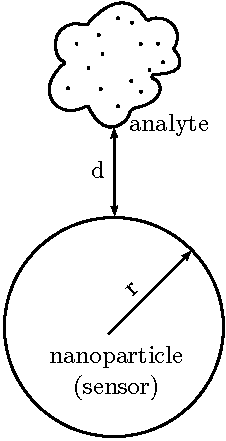
\includegraphics[width=0.15\textwidth]{protein_sphere_sketch.pdf} 
   \caption{Setup for convergence analysis of the response calculation.}
   \label{fig:setup_conv}
\end{figure}

These tests used the conditions and parameters for the isolated sphere simulation
presented in Section \ref{sec:verification}. The protein dielectric constant was
$2.7514 + 0.2860i$, which we extracted from the 
functional relationship provided by Phan, et al. \cite{PhanETal2013}, and the 
distance between the sensor and the analyte was $d=1 \, nm$. BSA was oriented such that
its dipole moment was aligned with the y-axis. The error calculations for Figure \ref{fig:error_sphere-bsa}
and Table \ref{table:err_bsa_sensor} use the Richardson extrapolated value of extinction cross-section as a
reference, $C_{ext}= 1778.7259 \, nm^2$.


\begin{figure}[h] %  figure placement: here, top, bottom, or page
   \centering
   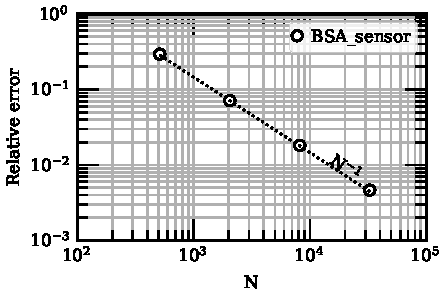
\includegraphics[width=0.45\textwidth]{convergence_bsa_sensor_R8_d=1_w=380.pdf} 
   \caption{Grid-convergence study of extinction cross-section of a spherical silver
            nanoparticle with a BSA protein at $d=1 \, nm$.}
   \label{fig:error_sphere-bsa}
\end{figure}

The observed order of convergence is $0.99$, and 
Figure \ref{fig:error_sphere-bsa} shows that the error decays with the number
of boundary elements ($1/N$), which is consistent with our verification 
results in Section \ref{sec:verification}. This proves that the
numerical solutions computed with \pygbe are correctly resolved by the meshes.
Also, the percentage errors for the different meshes are presented in Table. \ref{table:err_bsa_sensor}.

\begin{table}[h]
    \centering
    \caption{\label{table:err_bsa_sensor} Percentage error of BSA-sensor sytem (Fig.\ref{fig:setup_conv}) .} 
    \begin{tabular}{c c}
    \hline%\toprule
    N & \% error \\
    \hline%\midrule
     $512$ & $29.39$ \\
     $2048$ & $7.13$ \\
     $8192$ & $1.82$ \\
     $32768$ & $0.46$ \\
    \hline%\bottomrule
    \end{tabular}
\end{table}

\subsubsection{Resonance frequency shift calculations} \label{sec:bsa_shift}

We studied the LSPR response as a function of the wavelength in the presence 
of the BSA. To optimize run-times without compromising accuracy, we used a relaxed
set of parameters, where the protein mesh density was one element per
${\AA}^2$ ($N_{prot}=45140$) and the sphere mesh had $N_{sensor}=32768$. Integrals used
$K=4$ Gauss quadrature points for far-away elements, 
$K_{fine} = 19$ Gauss quadrature points in elements with near singular integrals,
and $Nk = 9$ Gauss quadrature points per triangle edge for the semi-analytical integration in the 
singular elements. The treecode used a Taylor expansion of order $P=6$ and a multipole-acceptance
criterion of $\theta=0.5$ . The GMRES tolerance was set to $10^{-3}$. 
This parameter choice resulted in a percentage error of $\sim\%0.6$
and the time of each computation was approximately $7.5 \, \text{min}$ in a \texttt{NVIDIA Tesla K40 GPU}
card when we have only one protein (when two proteins are present the time per run
is $\sim 15 \, \text{min}$). 

Figure \ref{fig:display_z} sketches the setup of the simulations, with two proteins placed 
$d=1 \, nm$ away from a spherical silver nanoparticle, along the z-axis.
The position of the BSA in the $+z$ axis was the same as the convergence analysis in 
Section \ref{sec:bsa_convergence}, whereas the BSA in the $-z$ position comes from a 180$^\circ$ 
solid rotation of the BSA in $+z$ about the y-axis.
We performed calculations for wavelengths between $382 \, nm$ and $387 \, nm$, every $0.25 \, nm$,
which are around the peak seen in Figure \ref{fig:verif_sphere}.

Figure \ref{fig:2pz_response} shows the variation of the extinction cross-section
with respect to wavelength for the isolated nanoparticle ($d=\infty$) and with
BSA proteins placed $d=1 \, nm$ away. 
Results present a red-shift ($0.5 \, nm$) in the resonance frequency due to the
presence of the BSA analytes.


\begin{figure}[h] %  figure placement: here, top, bottom, or page
   \centering
    %since we have dots in the names we need to enclose what is before the 
    %extension in { }
   \includegraphics[width=0.45\textwidth]{{2pz_00_ef-0.0037_R8nm}.pdf} 
   \caption{Extinction cross-section as a function of wavelength for a $8 \, nm$
            silver sphere immersed in water with two BSA proteins placed at
            $\pm 1 \; nm$ away from the surface in the z-direction, and at
            infinity (no protein).}
   \label{fig:2pz_response}
\end{figure}


To study the effect of location of the analytes, we reran simulations placing the 
BSA proteins along the x- and y-axis, at $\pm 1 \; nm$, as sketched by Figure \ref{fig:display_xy}.
Figure \ref{fig:2pxy_response} shows the results obtained for x-axis and
y-axis display, respectively. 

\begin{figure}[!h] %  figure placement: here, top, bottom, or page
   \centering
   \subfloat{\includegraphics[width=0.45\textwidth]{{2px_00_ef-0.0037_R8nm}.pdf}}
   \quad 
   \subfloat{\includegraphics[width=0.45\textwidth]{{2py_00_ef-0.0037_R8nm}.pdf}} 
   \caption{Extinction cross-section as a function of wavelength for a $8 \, nm$
            silver sphere immersed in water with two BSA proteins placed at
            $\pm 1 \; nm$ away from the surface in the x-direction (top) and
             y-direction (bottom), and at infinity (no protein).}
   \label{fig:2pxy_response}
\end{figure}

\subsubsection{Sensitivity calculations} \label{sec:bsa_sensitivity}

The sensitivity of an LSPR biosensor corresponds to the relation between the size 
of the resonance frequency shift and the number of analytes bound to the sensor (through a ligand).
Experiments show that the distance between the nanoparticle and the analyte largely
affects the sensitivity of the sensor, to the point that
targets placed $15nm$ away from the surface are very hard to detect \cite{HaesETal2004}.
This is a critical issue, considering that common ligands (for example, antibodies) are
larger than $15nm$. Figure \ref{fig:dist_response} 
shows how the peak varies with the distance at which the analytes ($+z$ and $-z$) are placed.  
In particular, we see a shift of $0.25 \, nm$ when $d=2 nm$ to $0.75 nm$ when the 
analytes are placed at $d=0.5 \, nm$. The parameters used in this case remain 
the same as the ones used in Figures \ref{fig:2pz_response} and \ref{fig:2pxy_response} .


\begin{figure}[h] %  figure placement: here, top, bottom, or page
   \centering
   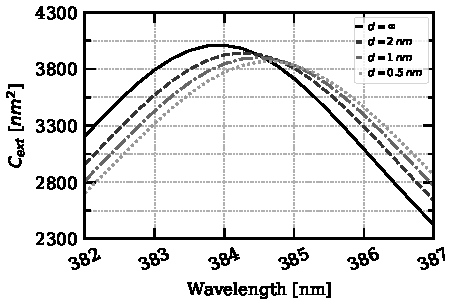
\includegraphics[width=0.45\textwidth]{2pz_lspr_response.pdf} 
   \caption{Extinction cross-section as a function of wavelength for a $8 \, nm$
            silver sphere immersed in water with two BSA proteins placed at
            $2, \, 1 \, \text{and} \, 0.5 \, nm$ away from the surface in the 
            z-direction, and at infinity (no protein)}
   \label{fig:dist_response}
\end{figure}

\begin{figure*}[] %  figure placement: here, top, bottom, or page
   \centering
   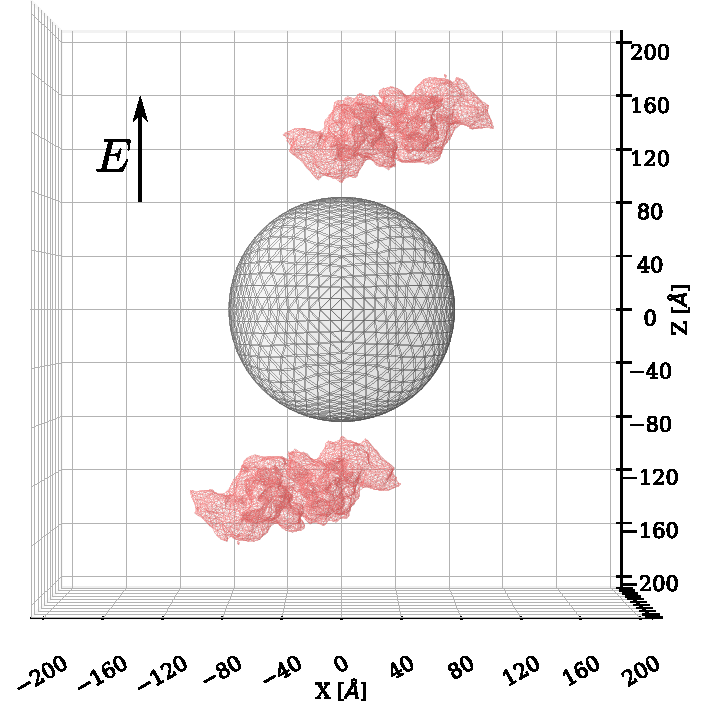
\includegraphics[width=0.65\textwidth]{2prot_1nm_z_R8nm.pdf} 
   \caption{Sensor protein display: BSA located at $\pm 1 \, nm$ of the 
            nanoparticle in the z-direction}
   \label{fig:display_z}
\end{figure*}

\begin{figure*}[]

   \centering
   \subfloat{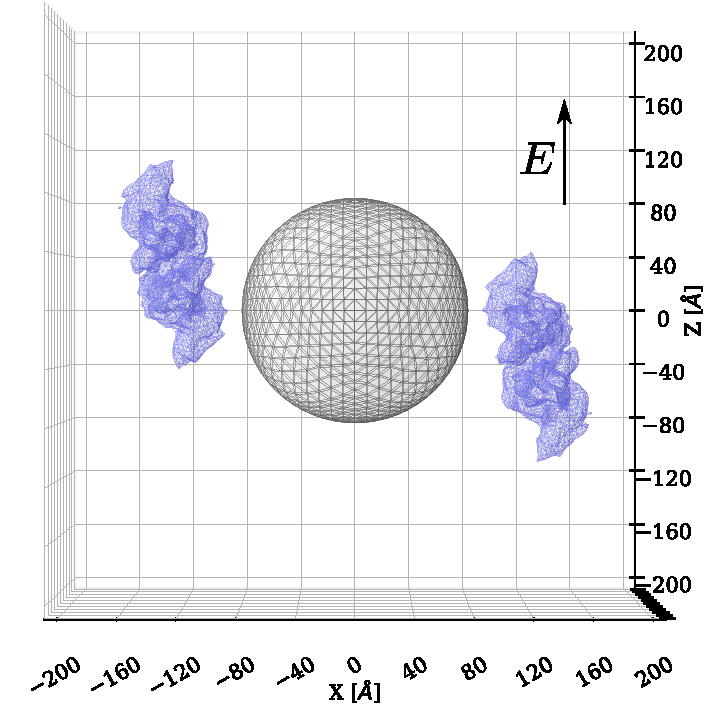
\includegraphics[width=0.65\textwidth]{2prot_1nm_x_R8nm.pdf}} 
%   \caption{Sensor protein display: BSA located at 1 nm of the nanoparticle in the
%            x-direction}
   %\label{fig:display_x}
    \vfill
   \subfloat{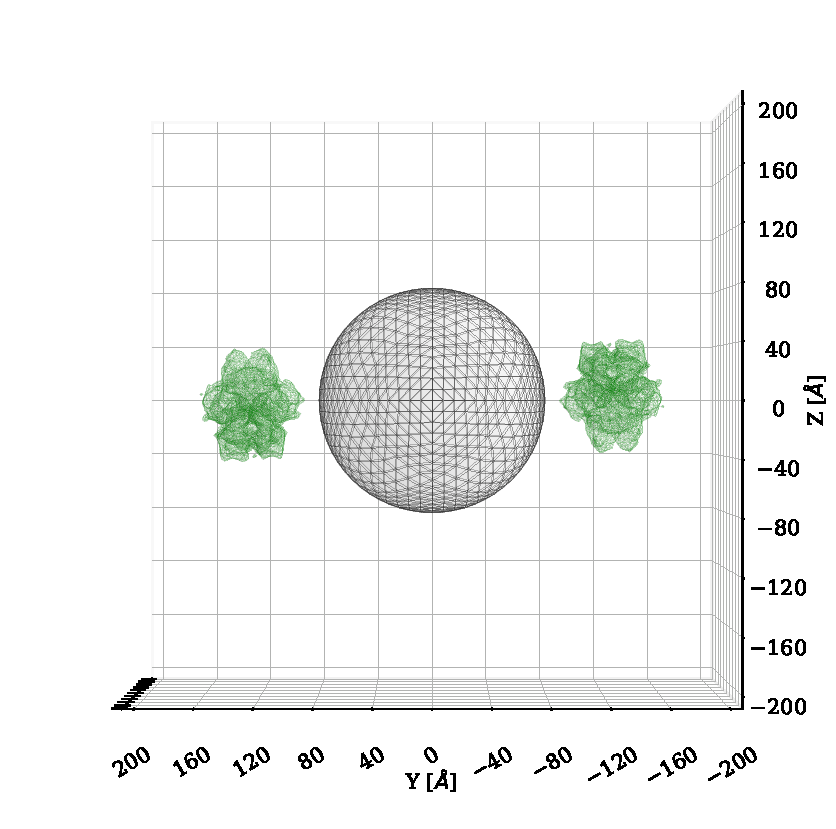
\includegraphics[width=0.65\textwidth]{2prot_1nm_y_R8nm.pdf}} 
%   \caption{Sensor protein display: BSA located at 1 nm of the nanoparticle in the
%            y-direction}
    \caption{Sensor protein display: BSA located at $\pm 1 \, nm$ of the nanoparticle in the
            x-direction (top) and y-direction (bottom)}
    \label{fig:display_xy}
\end{figure*}

\subsection{Reproducibility} \label{sec:repro}

We believe in reproducibility practices. To facilitate the replication of our results, 
we consistently release our code and data with every publication. \pygbe is developed and 
shared \footnote{\url{https://github.com/barbagroup/pygbe}} under the BSD3-clause 
license and the development repository is available on Github. We also release
all of the data and scripts needed to run the numerical simulations in this work, 
as well as the post-processing scripts to reproduce the figures in this paper. To be consistent with our open-source policy, we release a \textit{reproducibility package} for each of the results prensented in
this paper. {\color{red} explain location and which figure correspond to each package
after finished repropack}

